%! Author = kucera-lukas
%! Date = 4/12/22

\section{Uzivatel}\label{sec:uzivatel}

\subsection{Registrace}\label{subsec:registrace}
Na adrese \url{https://stegoer.netlify.app/account?form=register} (pokud neni
uzivatel jiz prihlasen) se zobrazi stranka, pomoci ktere je mozne si zalozit
novy uzivatelsky ucet.

Nalezitosti udaju noveho uzivatelskeho uctu:

\begin{enumerate}
    \item Uzivatelske jmeno musi mit alespon 6 znaku.
    \item Email musi odpovidat regulernimu vyrazu \verb/^\S+@\S+\.\S+$/.
    \item Heslo musi mit minimalne 6 znaku, obsahovat cislo, velke pismeno, male
    pismeno a alespon jeden specialni znak.
\end{enumerate}

\subsubsection{Zadavani hesla}\label{subsubsec:zadavani-hesla}

Pri vyplnovani se zobrazi popover\cite{enwiki:popover}, ktery uzivateli dava
najevo zda jeho heslo splnuje potrebne podminky.

\begin{figure}
    \centering
    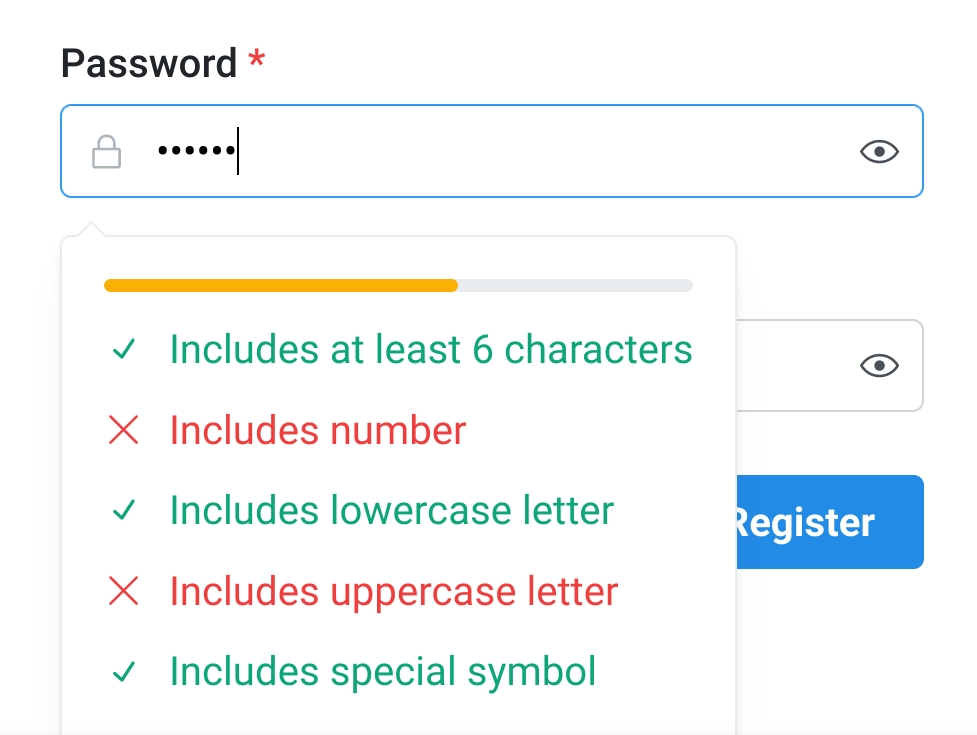
\includegraphics[scale=0.3]{assets/images/password-popover}
    \caption{Zadavani hesla}\label{fig:zadavani-hesla}
\end{figure}

\subsection{Prihlaseni}\label{subsec:prihlaseni}
Na adrese \url{https://stegoer.netlify.app/account?form=login} se zobrazi
prihlasovaci stranka.

Zde se pomoci emailu a hesla lze se prihlasit do vlastniho uctu (pokud neni
uzivatel jiz prihlasen).

U prihlaseni probiha kontrola pouze emailu, ktery by opet mel odpovidat
regulernimu vyrazu \verb/^\S+@\S+\.\S+$/.

\subsection{Sprava uctu}\label{subsec:sprava-uctu}
Pri kazdem vstupu na adresu \url{https://stegoer.netlify.app/account} aplikace
zkontroje stav uzivatele.

Pokud je uzivatel neni prihlasen aplikace ho presmeruje na prihlasovaci
stranku\ref{subsec:prihlaseni}

\subsubsection{Informace o uctu}

Z jednoduche tabulky, ktere se zobrazi hned pri vstupu lze vycist tri informace:

\begin{enumerate}
    \item Posledni datum prihlaseni uzivatele
    \item Posledni datum aktualizace uzivatele
    \item Datum vytvoreni uzivatelskeho uctu
\end{enumerate}

\subsubsection{Aktualizace uctu}

Prave tlacitko \texttt{Update account }otevre dialog pomoci ktereho muze
uzivatel zaktualizovat svuj ucet.

\paragraph{Zmena jmena a emailu}

Nabizi se zmena uzivatelskeho jmena, emailu a i hesla.
Samozrejme musi byt splneny stejne podminky jako pri registraci\ref{subsec:registrace}.

\paragraph{Zmena hesla}

Nabizi se zmena uzivatelskeho jmena, emailu a i hesla.
Samozrejme musi byt splneny stejne podminky jako pri registraci\ref{subsec:registrace}.

\subsubsection{Odhlaseni}

Po stisknuti leveho tlacitka \texttt{Logout} se uzivatel z jeho uctu odhlasi.

\subsection{Tabulka obrazku}\label{subsec:tabulka-obrazku}
Na adrese \url{https://stegoer.netlify.app/images} nalezneme tabulku, pomoci
ktere muze uzivatel prochazet obrazky, do kterych v minulosti ulozil nejaka
data.

\begin{figure}
    \centering
    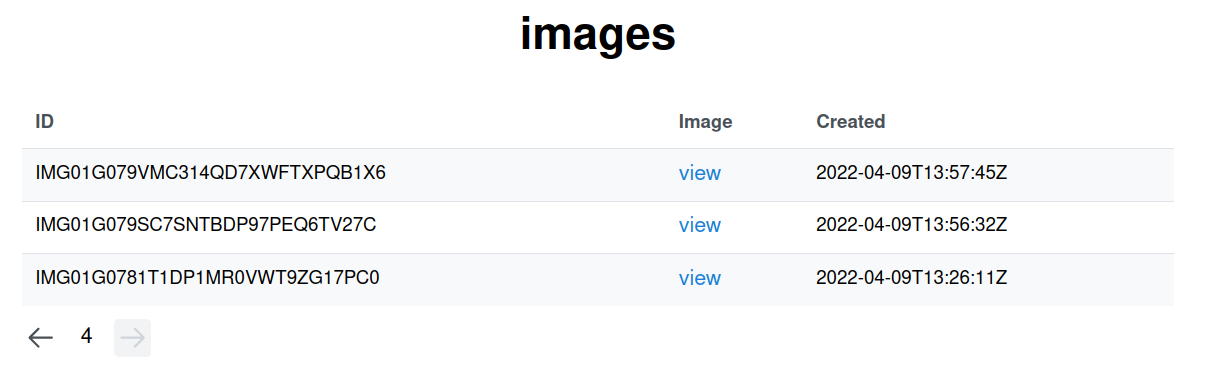
\includegraphics[scale=0.5]{assets/images/images-table}
    \caption{Tabulka s obrazky}\label{fig:tabulka-obrazky}
\end{figure}

\subsubsection{Strankovani}\label{subsubsec:strankovani}
Na jedne strane se zobrazi maximalne 10 radku, pro zobrazeni ostatnich je treba
pouzit navigacni tlacitka pod tabulkou.
Kazdy radek tabulky reprezentuje jeden obrazek a lze z neho vycist jeho ID a
datum vytvoreni.

\subsubsection{Detail obrazku}\label{subsubsec:detail-obrazku}
Tlacitko \texttt{view}, ktere se nachazi na kazdem radku slouzi k otevreni
detailni informace o souboru a moznost si obrazek opet znovu stahnout
(pokud tak uzivatel naucinil po zakodovani dat).

\begin{figure}
    \centering
    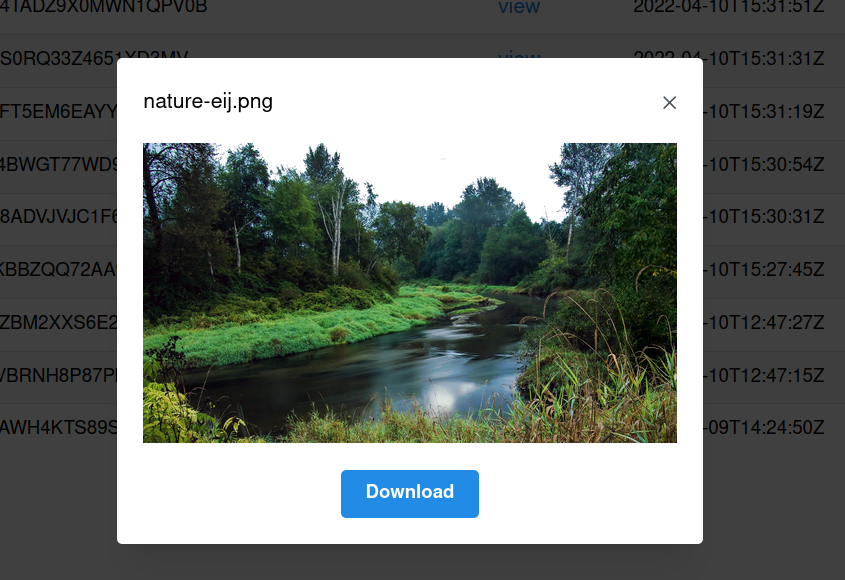
\includegraphics[scale=0.5]{assets/images/image-detail}
    \caption{Detailn obrazku}\label{fig:detail-obrazku}
\end{figure}
